\hypertarget{a00839}{}\section{Monolithic V\+Is and Effects}
\label{a00839}\index{Monolithic VIs and Effects@{Monolithic VIs and Effects}}
Extension of the \mbox{\hyperlink{a01481}{A\+A\+X\+\_\+\+C\+Effect\+Parameters}} class for monolithic V\+Is and effects. 

This extension to \mbox{\hyperlink{a01481}{A\+A\+X\+\_\+\+C\+Effect\+Parameters}} adds some conveniences for Virtual Instrument (VI) plug-\/ins and for other plug-\/ins that use a monolithic processing object, i.\+e. an object that combines state data with the audio render routine in a single object.

\begin{DoxyItemize}
\item The \mbox{\hyperlink{a01969_a04f2f73d70ea28c17747c68fc3a20fc8}{Render\+Audio}} method provides a direct audio processing callback within the data model object. Perform all audio processing in this method. \item The \mbox{\hyperlink{a01969_a69f9b80a70ecc6b7b2a7eec372d2502a}{Static\+Describe}} method establishes a generic M\+I\+DI processing context for the Effect. Call this method from the plug-\/in\textquotesingle{}s \mbox{\hyperlink{a00796}{Description callback}} implementation. \item The \mbox{\hyperlink{a01969_a1b23573e8aa3f8e64c61813b721559c2}{Add\+Synchronized\+Parameter}} method provides a mechanism for synchronizing parameter updates with the real-\/time thread, allowing deterministic, accurate automation playback. For more information abou this feature, see \mbox{\hyperlink{a00821_parameterUpdateTiming_sharedData}{Fixing timing issues due to shared data}}\end{DoxyItemize}
\begin{DoxyNote}{Note}
This convenience class assumes a monolithic processing environment (i.\+e. \mbox{\hyperlink{a00491_a0c5d795c1fd021c5b9b541febc34601aa027df08c137702400a92719828bea44b}{A\+A\+X\+\_\+e\+Constraint\+Location\+Mask\+\_\+\+Data\+Model}} .) This precludes the use of \mbox{\hyperlink{a01969}{A\+A\+X\+\_\+\+C\+Monolithic\+Parameters}} -\/derived Effects in distributed-\/processing formats such as A\+AX D\+SP.
\end{DoxyNote}
\mbox{\hyperlink{a01969}{A\+A\+X\+\_\+\+C\+Monolithic\+Parameters}} Collaboration diagram for Monolithic V\+Is and Effects\+:
\nopagebreak
\begin{figure}[H]
\begin{center}
\leavevmode
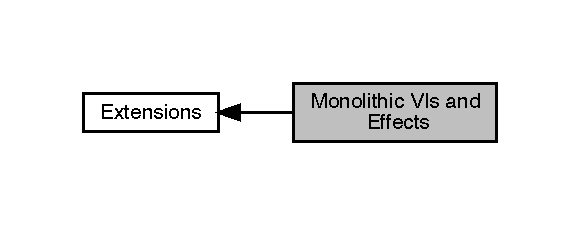
\includegraphics[width=279pt]{a00839}
\end{center}
\end{figure}
